% License: CC BY-SA
% Authors: See authors below and see also acknowledgement for authors of some images or research

\documentclass[25pt, margin=0mm, innermargin=15mm, blockverticalspace=15mm, colspace=15mm, subcolspace=8mm]{tikzposter}
\geometry{paperwidth=96in,paperheight=48in}

% to stretch boxes over whole paper with custor paper size
\makeatletter
\setlength{\TP@visibletextwidth}{\textwidth-2\TP@innermargin}
\setlength{\TP@visibletextheight}{\textheight-2\TP@innermargin}
\makeatother


\usepackage[utf8]{inputenc}
\usepackage{wrapfig}
\usepackage[hidelinks]{hyperref}

% For bibliography styling
%% TODO: all names should be abbreviated
\usepackage{natbib}

\definecolor{titleTextColor}{HTML}{009000}
\definecolorpalette{grassColorPalette} {
  \definecolor{colorOne}{HTML}{419041}
}
\usecolorstyle[colorPalette=grassColorPalette]{Britain}

\title{
\Huge
\textcolor{titleTextColor}{
\textsf{\textbf{
\fontsize{85}{60}\selectfont
How innovations thrive in GRASS GIS
}}
}
}

\newlength{\grasslogoheight}
\setlength{\grasslogoheight}{0.08\textheight}
\newlength{\instlogoheight}
\setlength{\instlogoheight}{0.35\grasslogoheight}

\titlegraphic{
\begin{minipage}{0.3\linewidth}

\includegraphics[height=\grasslogoheight]{grass}
\hspace{2em}

\includegraphics[height=\grasslogoheight]{osgeo_project}
\end{minipage}
\hfill
\begin{minipage}{0.15\linewidth}
\setlength{\baselineskip}{120pt}
\begin{flushright}

\includegraphics[height=\instlogoheight]{ncstate}
~

\includegraphics[height=\instlogoheight]{iwmi}
~

\includegraphics[height=\instlogoheight]{ctu_prague}
~

\includegraphics[height=\instlogoheight]{ti}
~

\includegraphics[height=\instlogoheight]{eurac}
~

\includegraphics[height=\instlogoheight]{mundialis}
~

\includegraphics[height=\instlogoheight]{fem_cri}
~

\includegraphics[height=\instlogoheight]{ec_jrc}
\end{flushright}
\end{minipage}
\vspace{-\grasslogoheight}
}

% \setlength{\blocktitleheight}{0.02\textheight}

% style for institute numbers
\newcommand{\inst}[1]{\hspace{2pt}$^{\mbox{\normalsize#1}}$\hspace{-7pt}}
\newcommand{\instlist}[1]{\hspace{1pt}$^{\mbox{\normalsize#1}}$\hspace{2pt}}

\author{
V\'{a}clav Petr\'{a}\v{s}\inst{1},
Yann Chemin\inst{2},
Martin Landa\inst{3},
Thomas Leppelt\inst{4},
S\"{o}ren Gebbert\inst{4},
Pietro Zambelli\inst{5},
Markus Neteler\inst{6},
Luca Delucchi\inst{7}, and
Margherita Di Leo\inst{8}
}
\institute{
\instlist{1}NCSU, USA;
\instlist{2}IWMI, Sri Lanka;
\instlist{3}FCE CTU in Prague, Czech Republic;
\instlist{4}TICSA, Germany;
\instlist{5}EURAC, Italy;
\instlist{6}mundialis GmbH \& Co. KG, Germany;
\instlist{7}CRI, FEM, Italy;
\instlist{8}EC-JRC, Italy
}

\hypersetup
{
    pdfauthor={V. Petras, Y. Chemin, M. Landa, S. Gebbert, P. Zambelli, M. Neteler, M. Di Leo},
    pdfsubject={},
    pdftitle={How innovations thrive in GRASS GIS},
    pdfkeywords={GIS, algorithms, methods, preservation, science, reproducibility}
}

% \usetemplate{1}
% \setinstituteshift{1}

% \setblocktitleheight{2}
% \setblockspacing{1}

\graphicspath{{images/}{logos/}}

\newcommand{\blocktitlewrap}[1]{\textsf{\textbf{\huge#1}}}
% it is not possible (?) to change block title in the class, using wrapper
% the command introduced using:
%   sed -i 's/\\block{\([^}]*\)}/\\block{\\blocktitlewrap{\1}}/g' main.tex

% GRASS module
\newcommand{\gmodule}[1]{\href{http://grass.osgeo.org/grass72/manuals/#1.html}{\emph{#1}}}
\newcommand{\gamodule}[1]{\href{http://grass.osgeo.org/grass72/manuals/addons/#1.html}{\emph{#1}}}
\newcommand{\gmodulenolink}[1]{\emph{#1}}

\begin{document}
\maketitle[width=0.92\textwidth]
% \maketitle
% \addlogo[north west]{(2,-1)}{9cm}{images/Grass_GIS}
%Please insert your institution logo here
% \addlogo[north east]{(-2,-2.5)}{4cm}{images/logo_FEM_CRI}
% \addlogo[north east]{(-2,-5.5)}{4cm}{images/NC_State_Seal}
% \addlogo[north east]{(-8,-2.5)}{4cm}{images/Logo_cvut}
% \addlogo[north east]{(-8,-6.5)}{4cm}{images/IWMI_logo}
% \addlogo[north east]{(-2,-10.5)}{4cm}{images/logo_ec-jrc}

\begin{columns}

%%%%%%%%%%%%%%%%%%%%%%%%%%%%%%%%%%%%%%%%%%%%%%%%%%%%%%%%%%%%%%%%%%%%%
%%%%%%%%%%%%%%%%%%%%%%%%%%%%%%%%%%%%%%%%%%%%%%%%%%%%%%%%%%%%%%%%%%%%%
%%%%%%%%%%%%%%%%%%%%%%%%%%%%%%%%%%%%%%%%%%%%%%%%%%%%%%%%%%%%%%%%%%%%%
%%%%%%%%%%%%%%%%%%%%%%%%%%%%%%%%%%%%%%%%%%%%%%%%%%%%%%%%%%%%%%%%%%%%%
\column{0.25}

%%%%%%%%%%%%%%%%%%%%%%%%%%%%%%%%%%%%%%%%%%%%%%%%%%%%%%%%%%%%%%%%%%%%%%%%%%%%%%%%
\block{\blocktitlewrap{Highlights}}
{
% \setlength{\parskip}{0.3ex}

\renewcommand{\labelitemi}{\textcolor{gray}{$\bullet$}\hspace{0.5ex}}

Poster topic highlights:

\begin{itemize}
 \item Algorithms and models included in GRASS GIS remain available long term \citep{chemin2015grass}.
 \item Analytical tools are not limited to one domain but spread across many fields.
 \item New tools can be build based on functionality or code of the existing ones
       regardless of the particular domain of problems they belong to.
 \item Both the functionality and the code are evaluated
       by the user and developer community in different fields of application beyond
       the field of expertise of the original authors
       and different scales of magnitude of data.
% continuous automated tests (Petras, 2014 \cite{Petras2014}),
\end{itemize}

General GRASS GIS highlights:

\begin{itemize}
%  \item Community supports users and new developments through online
%  \item long-term moving forward
 \item The GRASS GIS development team takes care of interface and operating system related changes
       in the code provided by scientists and contributors.
 \item Cost estimated by Black Duck Open Hub is over \$30,000,000.
 \item The free, libre and open source license used in GRASS GIS
       not only allows users to reduce GIS software costs to minimum,
       but also enables organizations to deploy cloud-based solutions without any license restrictions.
 \item GRASS GIS is used both directly and as a backend in other projects
       such as QGIS and R.
\end{itemize}

% oholoh hours

}


%%%%%%%%%%%%%%%%%%%%%%%%%%%%%%%%%%%%%%%%%%%%%%%%%%%%%%%%%%%%%%%%%%%%%
\block{\blocktitlewrap{Spatio-Temporal Data Analysis}}{
The time dimension was introduced in GRASS GIS version 7 for vector maps, rasters, and 3D rasters
which transformed GRASS GIS into a fully-featured temporal GIS \citep{Gebbert20141, gebbert2015grass}.
Time series of map layers are managed in space time datasets, a new data type in GRASS GIS,
and are still accessible also as individual map layers.
Based on the GRASS GIS Temporal Framework Python application programming interface (API),
more than 50 modules were implemented to manage, analyze, process
and visualize space time datasets.
More than 100,000 map layers can be now handled efficiently in GRASS GIS.
Example usages of this functionality include
analysis of the
European Climate Assessment \& Dataset ECA\&D \citep{Haylock2008_climate_series}
and temperate climate zone in the European Union identification \citep{Gebbert20141}.

The new temporal modules (staring with \gmodulenolink{t.})
work beside well established \gmodule{r.series} module
and specialized modules such as \gamodule{r.hants} implemented according to \cite{roerink2000reconstructing}
or \gamodule{r.seasons}.
Latest addition includes raster and vector temporal algebra
which can be used for tasks such as computing hydrothermal coefficient for a time series of climate data
using the actual mathematical formula \citep{leppelt2015grass}.

\vspace*{1cm}

\begin{minipage}{\linewidth}
\centering
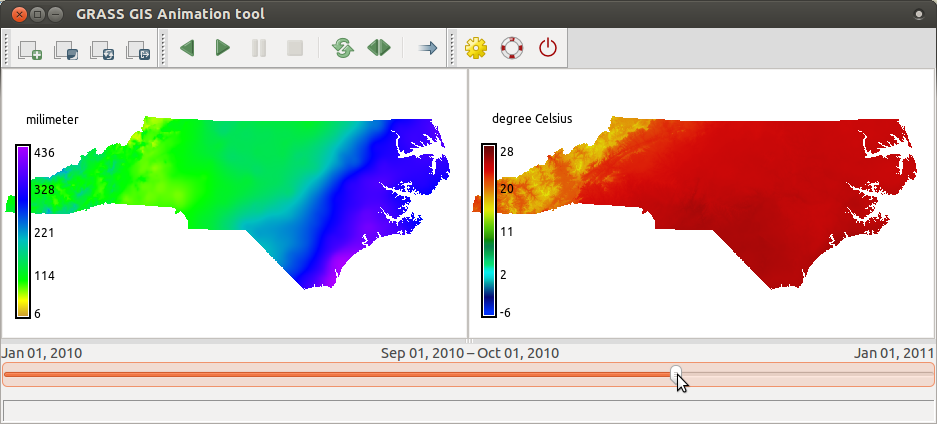
\includegraphics[width=.7\linewidth]{images/temporal_precip_temp}
\\
Creating a synchronized animation of monthly total precipitation and mean temperature for NC, USA
\end{minipage}

% \vspace*{1cm}

}


\block{\blocktitlewrap{Landscape Structure}}{
A set of modules for multiscale analysis of landscape structure was added in 1992
by \cite{baker1992r}, who developed the \gmodulenolink{r.le} model similar to
FRAGSTATS \citep{mcgarigal1995fragstats}.
The modules were gradually improved to become \gmodule{r.li} in 2006.
Further development continued, with a significant
increase in speed \citep{tracrli} and a new interactive user interface.
\cite{rocchini2013calculating} used \gmodule{r.li} modules to implement
high level tool for calculating landscape diversity.

\bigskip

\begin{minipage}{0.5\linewidth}
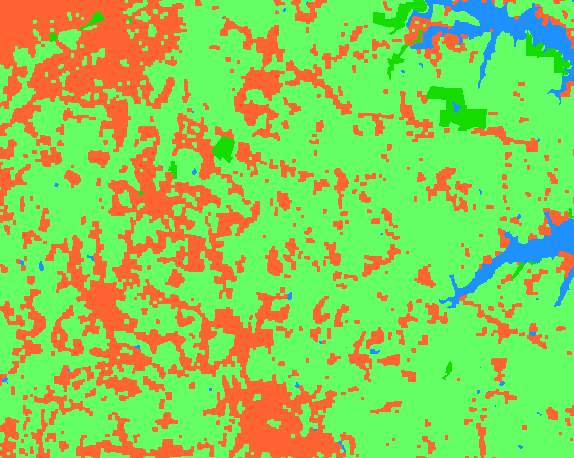
\includegraphics[width=\textwidth, trim={0 180 0 0}, clip]{diversity_classes}
\end{minipage}
\begin{minipage}{0.5\linewidth}
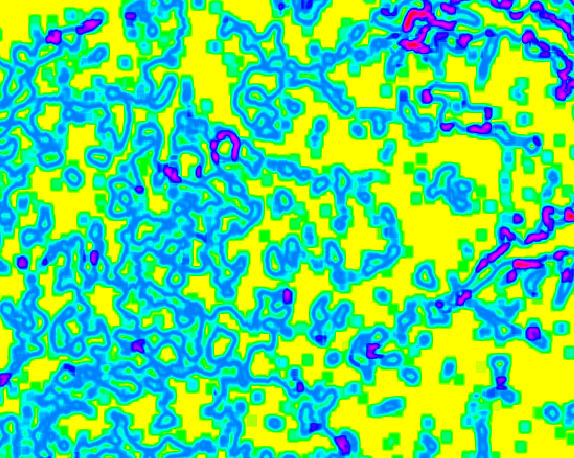
\includegraphics[width=\textwidth, trim={0 180 0 0}, clip]{diversity_shannon}
\end{minipage}

\medskip
Landuse classes and derived landscape diversity according to Shannon index in near Charlotte (NC, USA)
% r.diversity input=development_2006 prefix=diversity alpha=0.5 size=65
% r.li.shannon input="development_2006" config="conf_diversity_65.0" output="diversity_shannon_size_65.0"
}



%%%%%%%%%%%%%%%%%%%%%%%%%%%%%%%%%%%%%%%%%%%%%%%%%%%%%%%%%%%%%%%%%%%%%
%%%%%%%%%%%%%%%%%%%%%%%%%%%%%%%%%%%%%%%%%%%%%%%%%%%%%%%%%%%%%%%%%%%%%
%%%%%%%%%%%%%%%%%%%%%%%%%%%%%%%%%%%%%%%%%%%%%%%%%%%%%%%%%%%%%%%%%%%%%
%%%%%%%%%%%%%%%%%%%%%%%%%%%%%%%%%%%%%%%%%%%%%%%%%%%%%%%%%%%%%%%%%%%%%
\column{0.25}


%%%%%%%%%%%%%%%%%%%%%%%%%%%%%%%%%%%%%%%%%%%%%%%%%%%%%%%%%%%%%%%%%%%%%
%%%%%%%%%%%%%%%%%%%%%%%%%%%%%%%%%%%%%%%%%%%%%%%%%%%%%%%%%%%%%%%%%%%%%%%%%%%%%%%%%
\block{\blocktitlewrap{Water, Floods and Erosion}}{

GRASS GIS entails several modules that constitute the result of active research on natural hazards.
The \gmodule{r.sim.water} simulation model (Mitas and Mitasova, 1998 \cite{Mitas1998b})
for overland flow with spatially variable rainfall excess conditions was integrated into the Emergency
Routing Decision Planning system as a WPS (Raghavan et al., 2014 \cite{raghavan2014deploying}).
The module \gmodule{r.sim.water} together with
the module \gmodule{r.sim.sediment} for erosion-deposition modeling
implements a path sampling algorithm which is robust and easy to parallelize.
The \gmodule{r.sim.water} module was also utilized by Petrasova et al., 2014 \cite{Petrasova2014} and is now part of
\emph{Tangible Landscape}, a tangible GIS system, which also incorporated \gmodule{r.damflood},
a dam break inundation simulation \cite{cannata2012two}.

\bigskip

\vspace*{1cm}

\centering
\begin{minipage}{0.65\linewidth}
\centering
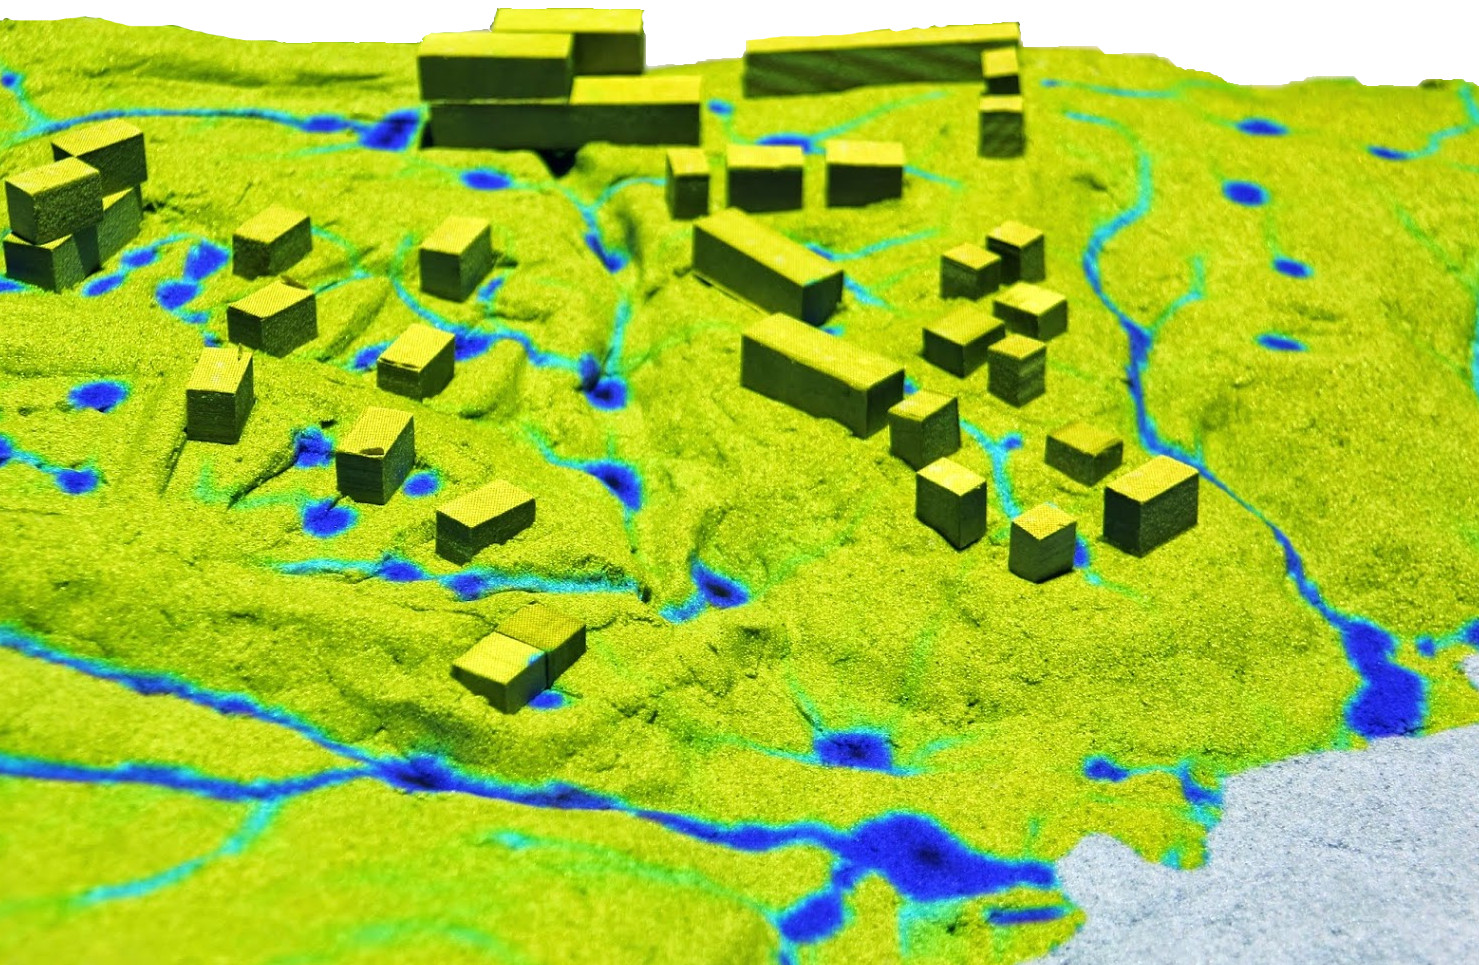
\includegraphics[width=0.5\textwidth]{rsimwater_architects}
\\
Overland flow simulated by \gmodule{r.sim.water} used for landscape
architecture design in Tangible Landscape environment
(Historical master plan for Lake Raleigh, NC, USA)
\end{minipage}
~
\begin{minipage}{0.5\linewidth}
% TODO: damflood on Lake Raleigh
% 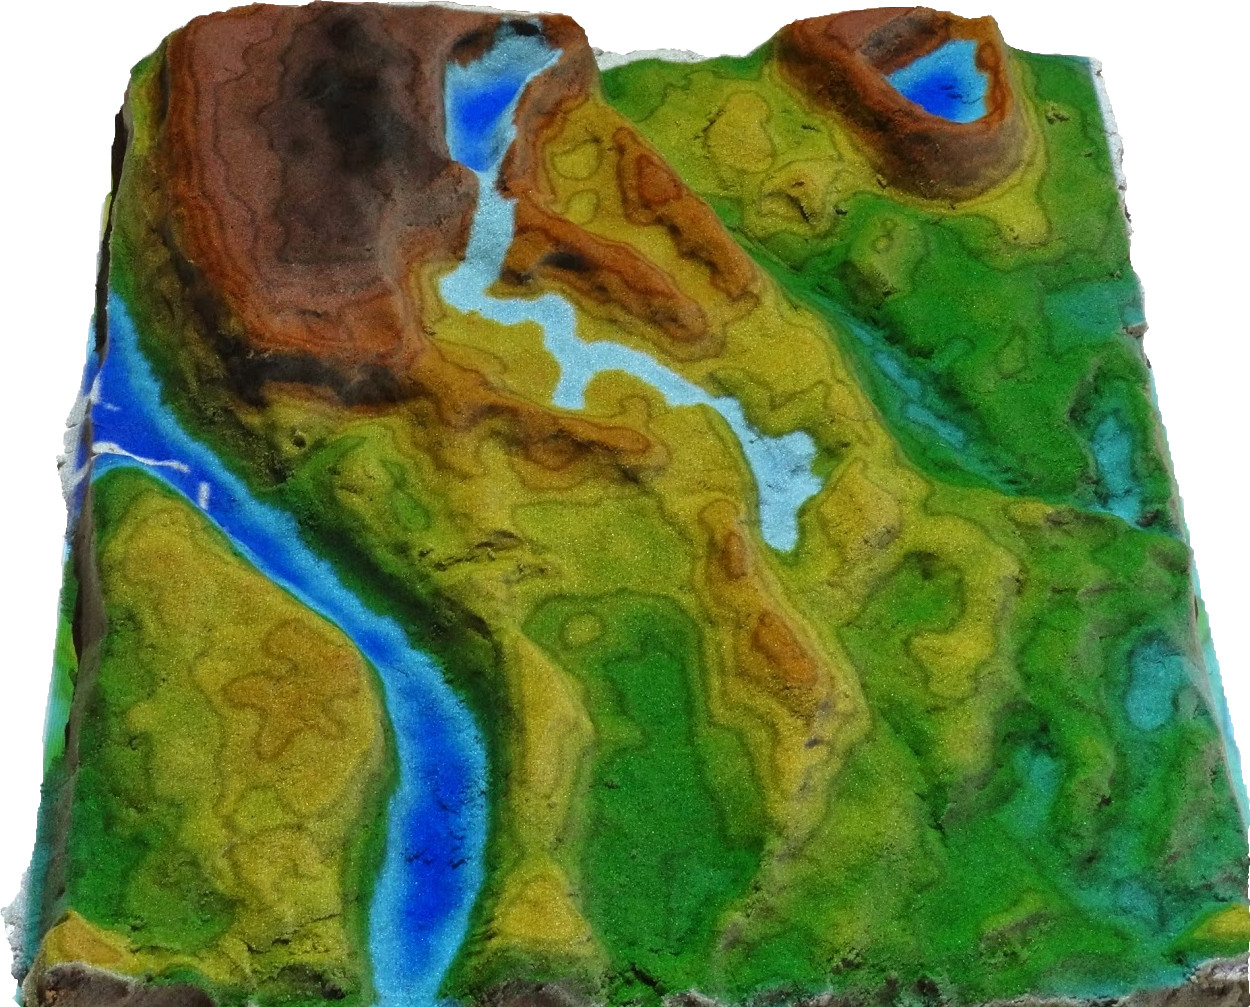
\includegraphics[width=\textwidth]{damflood_tangible}
% Coal ash pond breach in Tangible Landscape environment using \gamodule{r.damflood} module
\end{minipage}

% \vspace*{1.4cm}
}

%%%%%%%%%%%%%%%%%%%%%%%%%%%%%%%%%%%%%%%%%%%%%%%%%%%%%%%%%%%%%%%%%%%%%
\block{\blocktitlewrap{Lidar Data Processing}}{

Filtering of ground and non-ground points was included into GRASS GIS
early on in the lidar era in the \gmodule{v.lidar.edgedetection} group of modules.
% TODO: ref
% v.lidar.correction Corrects the v.lidar.growing output. It is the last of the three algorithms for LIDAR .
% v.lidar.edgedetection Detects the object's edges from a LIDAR data set.
% v.lidar.growing Building contour determination and Region Growing algorithm for determining the building inside
The module \gmodule{v.surf.rst} for spatial interpolation was developed approximately 20 years
ago, but since then it has been improved several times \cite{tracvsurfrst}
including recent parallelization which will be included in GRASS GIS 7.4.
Currently the module is used for both digital terrain model interpolation and interpolations in general.

The module \gmodule{r.in.lidar} statistically analyzes massive point clouds.
% TODO: base_raster, ref
For advanced general point analysis GRASS GIS
\gmodule{v.outlier} implemented originally specifically for lidar data
and recently also \gmodule{v.cluster}
implementing variety of clustering methods including
DBSCAN (Density-Based Spatial Clustering of Applications with Noise)
and OPTICS (Ordering Points to Identify the Clustering Structure).
The \gmodule{v.outlier} module serves as a base for a user contributed module \gamodule{v.lidar.mcc}
implementing MMC.
% TODO: ref

% v.delaunay v.voronoi New option to create Voronoi diagrams for areas.

\centering
\begin{minipage}{0.7\linewidth}
\centering
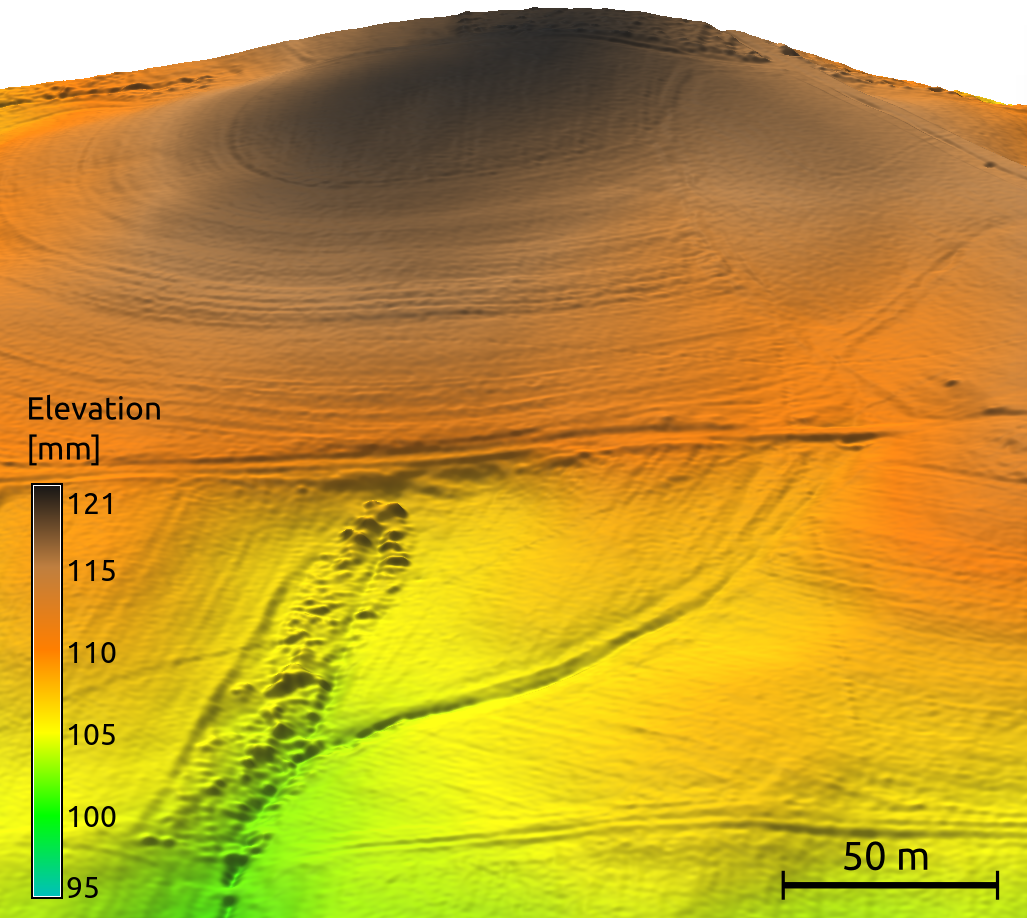
\includegraphics[width=0.5\textwidth]{elevation_lidar}
\\
Digital elevation model interpolated from LiDAR point clouds
using \gmodule{v.surf.rst}. Data are showing tillage in an agricultural field near Raleigh (North Carolina, USA)
\end{minipage}


}

%%%%%%%%%%%%%%%%%%%%%%%%%%%%%%%%%%%%%%%%%%%%%%%%%%%%%%%%%%%%%%%%%%%%
%%%%%%%%%%%%%%%%%%%%%%%%%%%%%%%%%%%%%%%%%%%%%%%%%%%%%%%%%%%%%%%%%%%%%
\column{0.25}

%%%%%%%%%%%%%%%%%%%%%%%%%%%%%%%%%%%%%%%%%%%%%%%%%%%%%%%%%%%%%%%%%%%%%%%%%%%%%%%
\block{\blocktitlewrap{Image Segmentations}}{
\gamodule{r.smooth.seg} (formerly \gmodulenolink{r.seg})
was created by Alfonso Vitti \citep{vitti2008free, vitti2012mumford}
and implemented a piece-wise smooth approximation of the original image
according to \cite{mumford1989optimal} and \cite{march1997variational}
which can be used to reduce noise in the original image.
This supplemented \gmodule{r.clump} available from 1980s
which groups pixes with same categories (or integer values).
The latest version of \gmodule{r.clump} coming in GRASS GIS 7.4
supports multiple image bands (or any rasters maps) as input.
Clumping of cells based on threshold value and clumping
of double precision floating point input is supported as well in the new version.

Eric Momsen implemented initial version of region-growing image segmentation in 2012
and Markus Metz then extended and optimized the code resulting in
the inclusion of the \gmodule{i.segment} module into GRASS GIS 7.0
and final replacement of old multi-resolution classification module of the same name
which was available in 1992 \citep{zhuang1992image}.
Another module called \gamodule{i.segment.hierarchical} by Pietro Zambelli is based on \gmodule{i.segment}
and performs parallelized hierarchical segmentation.

In 2016 GRASS GIS implementation of SLIC Superpixels segmentation \citep{achanta2010epfl, achanta2012slic}
was requested by the community
and Rashad Kanavath and Markus Metz implemented \gmodule{i.superpixels.slic}
which provides users both with SLIC and SLIC0 methods.

\bigskip

\vspace*{1cm}

\begin{minipage}{0.5\linewidth}
\begin{center}
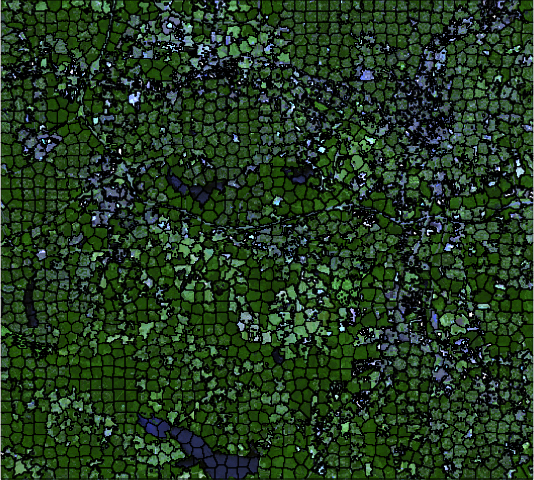
\includegraphics[width=\textwidth]{superpixels_slic_pseudo}
\end{center}
\end{minipage}
~
\begin{minipage}{0.5\linewidth}
\begin{center}
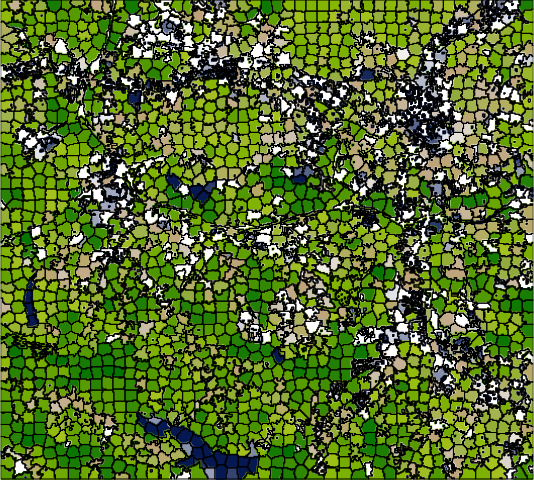
\includegraphics[width=\textwidth]{superpixels_slic_colored}
\end{center}
\end{minipage}
\vspace{2mm}
\begin{center}
Superpixels (back outlines) on pseudo-color image of central Wake county, NC, USA (left)
and same superpixels colored according to a mean NDVI value per pixel (right).
\end{center}

\vspace*{0.6cm}

}


%%%%%%%%%%%%%%%%%%%%%%%%%%%%%%%%%%%%%%%%%%%%%%%%%%%%%%%%%%%%%%%%%%%%%%%%%%%%%%%%
\block{\blocktitlewrap{Topology, Cleaning, Overlays, Attributes}}{
Besides basic vector analysis tools such as \gmodule{v.buffer}
and \gmodule{v.overlay},
% TODO: v.overlay: The processing speed has been substantially improved

cleaning (also v.build error
% + clustering + neighorhood + vector algebra

v.feature.algebra (formerly v.mapcalc) replaced by Python for GRASS GIS C libraries (PyGRASS)

Attribute processing and queries in GRASS GIS can take an advantage of latest developments
in database management systems (DBMSs) as several DBMSs are supported most notably SQLite and PostgreSQL.

Non-topological vector
data are automatically converted to a topological representation upon import. Further more, various cleaning tools exist
to remove non-trivial topological errors.

The GRASS GIS 7 releases come with faster vector processing backend
and more efficient internal vector format;
both disk and memory requirements were reduced.
The new spatial index performs queries faster (more than 10 times for large vectors compared to GRASS GIS 6).

All topological cleaning tools have been optimized with regard to processing speed, robustness, and system
requirements.

Considering the wide spread usage of Esri Shapefile, a non-topological format for vector data exchange, it is particularly
advantageous that GRASS GIS 7 offers advanced cleaning tools.

postgis incl topo
GRASS GIS 7 supports various data sources in read and write access. Beside native file-based raster and vector format
GRASS allows to specify external data sources through GDAL/OGR library. GRASS GIS 7 also natively supports
PostGIS database including its topological extension.

In parallel to that native support the OGC Simple Features was added.

\centering
\begin{minipage}{0.9\linewidth}
\begin{center}
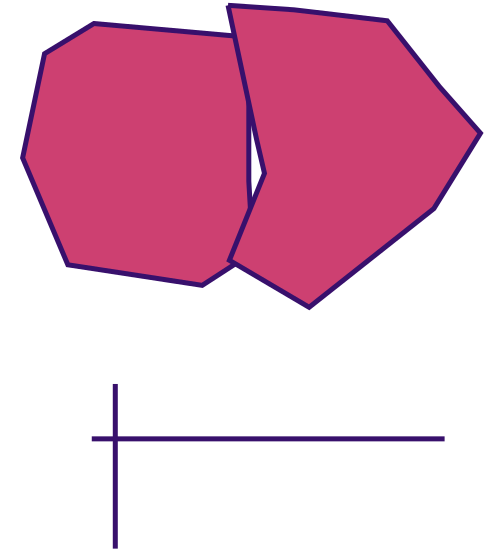
\includegraphics[width=.3\textwidth]{topo_original}
~
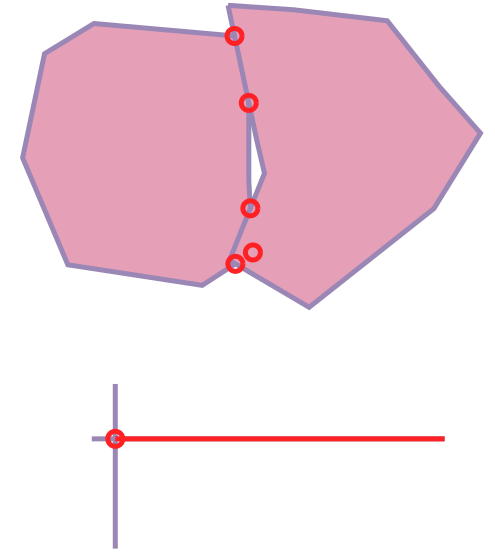
\includegraphics[width=.3\textwidth]{topo_errors}
~
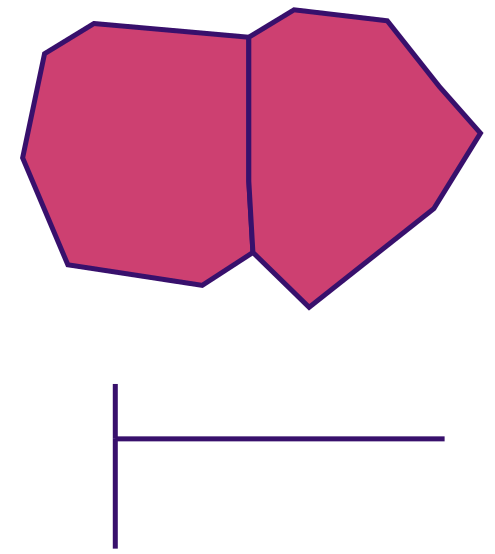
\includegraphics[width=.3\textwidth]{topo_fixed}
Original vector imported without cleaning (left),
identified errors (middle),
automatically topologically corrected vector (right)
\end{center}
\end{minipage}

% v.in.ascii input= output=imported format=standard
% v.build -e map=imported error=errors
% v.clean -c input=imported output=clean error=cleaning_errors tool=snap,rmdangle,rmbridge,chbridge,bpol,prune threshold=5
% d.vect map=cleaning_errors color=255:33:36 fill_color=none width=5 icon=basic/point size=30
% d.vect map=imported color=56:16:108 fill_color=205:64:113 width=5

}

%%%%%%%%%%%%%%%%%%%%%%%%%%%%%%%%%%%%%%%%%%%%%%%%%%%%%%%%%%%%%%%%%%%%%
%%%%%%%%%%%%%%%%%%%%%%%%%%%%%%%%%%%%%%%%%%%%%%%%%%%%%%%%%%%%%%%%%%%%%
%%%%%%%%%%%%%%%%%%%%%%%%%%%%%%%%%%%%%%%%%%%%%%%%%%%%%%%%%%%%%%%%%%%%%
%%%%%%%%%%%%%%%%%%%%%%%%%%%%%%%%%%%%%%%%%%%%%%%%%%%%%%%%%%%%%%%%%%%%%
\column{0.25}


%%%%%%%%%%%%%%%%%%%%%%%%%%%%%%%%%%%%%%%%%%%%%%%%%%%%%%%%%%%%%%%%%%%%%%%%%%%%%%%%
\block{\blocktitlewrap{Vector Network Analysis}}{
All vector network analysis tools provide now fine control over node costs.

\centering
\begin{minipage}{0.5\linewidth}
\begin{center}
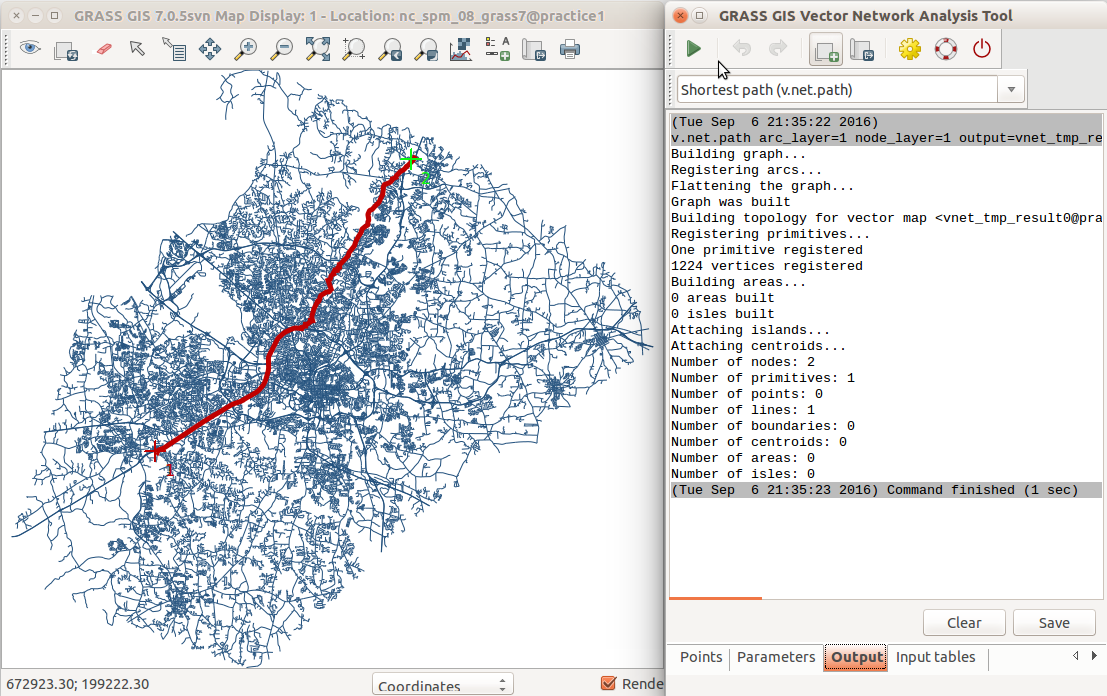
\includegraphics[width=\textwidth]{network}
Shortest path between two points in the Wake County road network (NC, USA)
\end{center}
\end{minipage}

}


%%%%%%%%%%%%%%%%%%%%%%%%%%%%%%%%%%%%%%%%%%%%%%%%%%%%%%%%%%%%%%%%%%%%%%%%%%%%%%%%
\block{\blocktitlewrap{References}}{

\vspace{-0.2cm}
\scriptsize

% \newcommand{\blocksectiontitle}[1]{\subsubsection*{\textcolor{gray}{\textsf{#1}}}}
\newcommand{\blocksectiontitle}[1]{\textbf{#1}}

%\blocksectiontitle{References}
\begingroup
\renewcommand{\section}[2]{}%
\bibliographystyle{apalike}
\bibliography{poster}
\endgroup

}


%%%%%%%%%%%%%%%%%%%%%%%%%%%%%%%%%%%%%%%%%%%%%%%%%%%%%%%%%%%%%%%%%%%%%%%%%%%%%%%%
\block{\blocktitlewrap{Acknowledgements}}{

\newcommand{\listhspace}{\hspace{0.005\linewidth}}
\newcommand{\listlogowidth}{0.10\linewidth}
\newcommand{\listtextwidth}{0.82\linewidth}

\begin{minipage}{\listlogowidth}

\includegraphics[width=\linewidth]{osgeo}
\end{minipage}
\listhspace
\begin{minipage}{\listtextwidth}
Open Source Geospatial Foundation (OSGeo)
supports the collaborative development of open source geospatial software.
GRASS GIS is a OSGeo project.
OSGeo provides infrastructure for project
websites, mailing lists and source code management.
\end{minipage}

\bigskip

\begin{minipage}{\listlogowidth}

\includegraphics[width=\linewidth]{google}
\end{minipage}
\listhspace
\begin{minipage}{\listtextwidth}
Initial development of \gmodule{i.segement} module as well as several other developments
were done as a part of the Google Summer of Code project.
Google provides financial support to students and organizations participating in the Google Summer of Code project.
\end{minipage}

\bigskip

\vspace{0.2cm}

\textcolor{gray}{
\hrulefill
}

\vspace{0.1cm}

\newcommand{\qrcodesize}{0.05\linewidth}

% qrencode http://grass.osgeo.org -o qr_grass.eps -t EPS
% epspdf -b qr_grass.eps qr_grass.pdf

\begin{center}
\begin{tabular}{c}

% \hspace{5mm}

\begin{minipage}{\qrcodesize}

\includegraphics[width=\textwidth]{./images/qr_grass.pdf}
\end{minipage}
~
\begin{minipage}{0.15\linewidth}
\small {\href{http://grass.osgeo.org}{\nolinkurl{grass.osgeo.org}}}
\end{minipage}

\begin{minipage}{0.1\linewidth}
\href{http://creativecommons.org/licenses/by-sa/4.0/}{
\includegraphics[width=\textwidth]{ccbysa}}
\end{minipage}
~
\begin{minipage}{0.35\linewidth}
\small This poster is licensed under a Creative Commons Attribution-ShareAlike 4.0 International License.
\end{minipage}

\end{tabular}
\end{center}

\vspace{-0.08cm}
}

\end{columns}

\end{document}
